\documentclass[pdftex,
	a4paper,
	titlepage=false]{scrreprt}
\usepackage[utf8]{inputenc}       
\usepackage[T1]{fontenc}
\usepackage{graphicx}
\usepackage{xcolor}
\usepackage{booktabs} % table rulers
\usepackage{longtable} % multipage tables
\usepackage{todonotes}
\usepackage{amsmath}
\usepackage{float} % for [H]
\usepackage{array, ragged2e}
\newcolumntype{R}[1]{>{\RaggedLeft\arraybackslash}p{#1}} % right aling column with fixed width

% Continuous figure counting (instead of per cahpter)
\usepackage{chngcntr}
\counterwithout{figure}{chapter}
\counterwithout{table}{chapter}
% Add 'S' before figure/table numbering
\renewcommand{\thefigure}{S\arabic{figure}}
\renewcommand{\thetable}{S\arabic{table}}
\renewcommand{\thepage}{S\arabic{page}}

\usepackage[
	round,	%(defaultage in the main file and \input ) for round parentheses;
	authoryear,% (default) for author-year citations;
	sort,		% orders multiple citations into the sequence in which they 
]{natbib}	


% affiliations
\usepackage[affil-it]{authblk}

% counts
% http://ctan.mackichan.com/macros/latex/contrib/caption/totalcount.pdf
\usepackage[figure,table, page]{totalcount}



%% -------------------------------------------------------------------------
\title{Supplemental Materials for: \\ Large scale risks from pesticides in small streams}
\author{Eduard Szöcs%
  \thanks{Corresponding author, Email: \texttt{szoecs@uni-landau.de}}}
\affil[1]{Institute for Environmental Sciences, University of Koblenz-Landau, Germany}

\author{Marvin Brinke}
\affil{German Federal Institute of Hydrology (BfG), Koblenz, Germany}

\author{Bilgin Karaoglan}
\affil{German Environment Agency (UBA), Dessau-Roßlau, Germany}

\author[1]{Ralf B. Schäfer}


%% -------------------------------------------------------------------------
\begin{document}
\maketitle

\vfill
\begin{description}
	\item[Number of pages: ] \totalpages
	\item[Number of figures: ] \totalfigures
	\item[Number of tables: ] \totaltables
\end{description}
% increase page counter by 1
\setcounter{page}{2}

\tableofcontents
\listoffigures
\listoftables



%% -------------------------------------------------------------------------
\chapter{Data Cleaning}
Before combining into a common database, more than 30 datasets have been cleaned and homogenised separately.
Cleaning steps comprised the following steps (Figure~\ref{fig:data_cleaning} gives a graphical overview):

\begin{enumerate}
	\item Structure: Datasets have been adjusted to the database structure.
	\item Coordinates: Coordinates have been transformed to a common Coordinate Reference System (DHDN / 3-Grad Gauss-Krüger Zone 3 (EPSG:31467)) and duplicates merged.
	\item Chemicals: Chemical names and identifiers have been unified using the webchem package (https://github.com/ropensci/webchem).
	\item  Identifiers: Unique identifiers have been assigned.
	\item Units: All concentrations have been converted to $\mu g/L$. Values below limit of quantification were set to zero (and can be used to identify non-detects).
	\item Other meta-data: meta-data has been standardised.
	\item Temporal resolution: The temporal resolution of the database is 1 day. Samplings below this resolution have been aggregated by the maximum daily value.
	\item Validity Checks: Simple rules for validity checks have been implemented.
\end{enumerate}

\begin{figure}[ht]
	\centering
	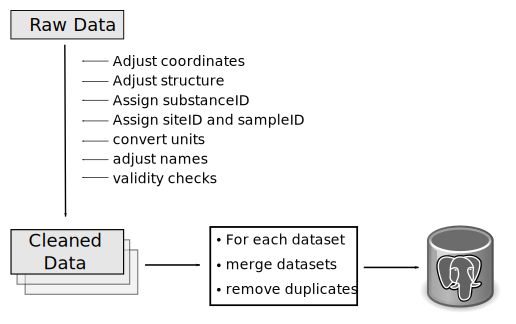
\includegraphics[width = 0.8\textwidth]{data_cleaning}
	\caption[Overview on data cleaning steps.]{Overview on data cleaning steps. After cleaning, data have been stored in a relational spatial PostgreSQL database.}
	\label{fig:data_cleaning}
\end{figure}



%% -------------------------------------------------------------------------
\chapter{Overview on compiled data}
% Overview samples
% table generated in do_overview.R
\begin{table}[ht]
\centering
\caption{Overview on chemical samples. Only data from running waters and grab
sampling is shown. \textsuperscript{a}: Abbreviations according to ISO 3166-2:DE. 
      \textsuperscript{b}: Including metabolites} 
\label{tab:phch_overview}
\begin{tabular}{lllrrr}
  \toprule
state \textsuperscript{a} & begin & end & no.sites & no.samples & no.compounds \textsuperscript{b} \\ 
  \midrule
BW & 2005-03-10 & 2014-10-02 & 7 & 172 & 98 \\ 
  BY & 2006-04-19 & 2013-12-17 & 13 & 218 & 155 \\ 
  HE & 2007-01-15 & 2014-12-18 & 65 & 2411 & 144 \\ 
  MV & 2005-03-08 & 2014-12-17 & 130 & 1503 & 227 \\ 
  NI & 2014-03-24 & 2014-10-13 & 1 & 7 & 226 \\ 
  NW & 2005-01-18 & 2015-01-22 & 1139 & 8536 & 198 \\ 
  RP & 2008-01-02 & 2013-12-18 & 7 & 341 & 236 \\ 
  SH & 2005-04-26 & 2014-11-26 & 269 & 1380 & 180 \\ 
  SL & 2005-01-03 & 2013-11-25 & 2 & 104 & 57 \\ 
  SN & 2005-01-02 & 2013-12-18 & 606 & 9141 & 173 \\ 
  ST & 2005-01-24 & 2015-03-19 & 30 & 416 & 88 \\ 
  TH & 2005-06-16 & 2014-12-08 & 32 & 514 & 63 \\ 
   \midrule
Total & 2005-01-02 & 2015-03-19 & 2301 & 24743 & 478 \\ 
   \bottomrule
\end{tabular}
\end{table}


\begin{figure}[ht]
	\centering
	\includegraphics[width = \textwidth]{temporal}
	\caption{Number of sampling occasions per year and month.}
	\label{fig:temporal}
\end{figure}

% \begin{figure}[ht]
% 	\centering
% 	\includegraphics[width = 0.8\textwidth]{varclus}
% 	\caption[Complete Linkage Cluster Dendrogram of Jaccard Similarity of analysed compound spectra between federal states.]{Complete Linkage Cluster Dendrogram of Jaccard Similarity of analysed compound spectra between federal states. Abbreviations of state names according to ISO 3166-2:DE (see also Table~\ref{tab:phch_overview}).}
% 	\label{fig:varclus}
% \end{figure}

% \begin{figure}[ht]
% 	\centering
% 	\includegraphics[width = 0.6\textwidth]{silhouette}
% 	\caption[Average silhouette width for different cluster sizes.]{Average silhouette width for different cluster sizes of complete linkage clustering of jaccard similarity of analysed compound spectra between federal states. Two clusters showed the maximum silhouette width.}
% 	\label{fig:silhouette}
% \end{figure}

% Overview variables
% table generated in do_overview.R
\newpage
\begingroup\fontsize{8pt}{10pt}\selectfont
\begin{longtable}{lp{3cm}rlp{0.5cm}p{0.5cm}p{1.5cm}p{1cm}p{1cm}p{1cm}}
\caption{Analysed chemical compounds. \
                    \textsuperscript{a} Authorized in Germany (Source: BVL, 2015). 
                    \textsuperscript{b} Authorized in the EU (Source: EU).
                    \textsuperscript{c} [ug/L].
                    \textsuperscript{d} chemprop: Read-Across \citep{schuurmann_quantitative_2011};
                                         epa: US EPA \citep{u.s._epa_ecotoxicology_2015};
                                         malaj:\citep{malaj_organic_2014};
                                         ppdb: Pesticides Properties database \citep{lewis_international_2016};
                                         none: no LC50 could be found.
                    \textsuperscript{e} Maximum Anual Concentration Environmental Quality Standard [ug/L].
                    \textsuperscript{f} Regulatory Acceptable Concentration [ug/L] (Source: German EPA).} \\ 
  \toprule
 & Name & CAS & Group & Auth. GER\textsuperscript{a} & Auth. EU\textsuperscript{b} & LC50\textsubscript{D.magna}\textsuperscript{c} & Source LC50\textsuperscript{d} & MAC-EQS\textsuperscript{e} & RAC \textsuperscript{f} \\ 
  \midrule
1 & 1,3-cis-Dichlorpropen & 10061-01-5 & other &  &  & 6483.44 & chemprop &  &  \\ 
  2 & 1,3-trans-Dichlorpropen & 10061-02-6 & other &  &  & 6483.44 & chemprop &  &  \\ 
  3 & 2,4-D & 94-75-7 & herbicide & x & x & 148281.00 & malaj & 1.00 & 1.10 \\ 
  4 & 2,4-DB & 94-82-6 & herbicide &  & x & 25000.00 & malaj &  &  \\ 
  5 & 2,4-Dichlorphenol & 120-83-2 & metabolite &  &  & 2600.00 & malaj &  &  \\ 
  6 & 2,4,5-T & 93-76-5 & herbicide &  &  & 5000.00 & malaj &  &  \\ 
  7 & 2,4,6-Trichlorphenol & 88-06-2 & metabolite &  &  & 1710.00 & malaj &  &  \\ 
  8 & 2,6-Dichlorobenzamid & 2008-58-4 & metabolite &  &  & 180000.00 & malaj &  &  \\ 
  9 & 3-Hydroxy Carbofuran & 16655-82-6 & metabolite &  &  & 293.44 & chemprop &  &  \\ 
  10 & 4,6-Dinitro-o-Cresol & 534-52-1 & insecticide &  &  & 3200.00 & malaj &  &  \\ 
  11 & Acetochlor & 34256-82-1 & herbicide &  &  & 8600.00 & malaj &  &  \\ 
  12 & Acetochlorsäure & 194992-44-4 & metabolite &  &  &  & none &  &  \\ 
  13 & Acetochlorsulfonsäure & 187022-11-3 & metabolite &  &  & 139523.68 & chemprop &  &  \\ 
  14 & Aclonifen & 74070-46-5 & herbicide & x & x & 1200.00 & ppdb & 0.12 & 1.06 \\ 
  15 & Alachlor & 15972-60-8 & herbicide &  &  & 10000.00 & malaj & 0.70 &  \\ 
  16 & Aldicarb & 116-06-3 & insecticide &  &  & 339.52 & epa &  &  \\ 
  17 & Aldrin & 309-00-2 & insecticide &  &  & 28.00 & malaj &  &  \\ 
  18 & Ametryn & 834-12-8 & herbicide &  &  & 28000.00 & malaj &  &  \\ 
  19 & AMPA & 1066-51-9 & metabolite &  &  &  & none &  &  \\ 
  20 & Atrazin & 1912-24-9 & herbicide &  &  & 54000.00 & malaj & 2.00 &  \\ 
  21 & Atrazin, 2-Hydroxy & 2163-68-0 & metabolite &  &  & 36738.13 & chemprop &  &  \\ 
  22 & Avermectin B1a & 71751-41-2 & insecticide & x & x &  & none &  &  \\ 
  23 & Azinphos-ethyl & 2642-71-9 & insecticide &  &  & 4.00 & epa &  &  \\ 
  24 & Azinphos-methyl & 86-50-0 & insecticide &  &  & 2.09 & epa &  &  \\ 
  25 & Azoxystrobin & 131860-33-8 & fungicide & x & x & 254.47 & epa &  & 0.55 \\ 
  26 & Benalaxyl & 71626-11-4 & fungicide & x & x & 590.00 & ppdb &  & 20.00 \\ 
  27 & Bensulfuron-methyl & 83055-99-6 & herbicide &  & x & 130000.00 & ppdb &  &  \\ 
  28 & Bentazon & 25057-89-0 & herbicide & x & x & 125000.00 & malaj &  & 710.00 \\ 
  29 & Bifenox & 42576-02-3 & herbicide & x & x & 350.00 & epa & 0.04 &  \\ 
  30 & Bifenthrin & 82657-04-3 & insecticide &  & x & 1.53 & epa &  &  \\ 
  31 & Boscalid & 188425-85-6 & fungicide & x & x & 5330.00 & ppdb &  & 12.50 \\ 
  32 & Bromacil & 314-40-9 & herbicide &  &  & 121000.00 & malaj &  &  \\ 
  33 & Bromocyclen & 1715-40-8 & insecticide &  &  & 700.00 & ppdb &  &  \\ 
  34 & Bromoxynil & 1689-84-5 & herbicide & x & x & 12500.00 & malaj &  & 3.30 \\ 
  35 & Carbendazim & 10605-21-7 & fungicide &  &  & 131.52 & epa & 0.70 & 0.15 \\ 
  36 & Carbofuran & 1563-66-2 & insecticide &  &  & 9.40 & malaj &  &  \\ 
  37 & Chlordan & 57-74-9 & insecticide &  &  & 98.40 & malaj &  &  \\ 
  38 & Chlorfenvinphos & 470-90-6 & insecticide &  &  & 0.25 & malaj & 0.30 &  \\ 
  39 & Chloridazon & 1698-60-8 & herbicide & x & x & 132000.00 & malaj &  & 56.00 \\ 
  40 & Chloroxuron & 1982-47-4 & herbicide &  &  & 2950.00 & epa &  &  \\ 
  41 & Chlorpyrifos & 2921-88-2 & insecticide &  & x & 0.10 & malaj & 0.10 & 0.00 \\ 
  42 & Chlortoluron & 15545-48-9 & herbicide & x & x & 67000.00 & ppdb &  & 2.30 \\ 
  43 & Clomazon & 81777-89-1 & herbicide & x & x & 5200.00 & epa &  & 5.70 \\ 
  44 & Clopyralid & 1702-17-6 & herbicide & x & x & 225000.00 & malaj &  & 1080.00 \\ 
  45 & Clothianidin & 210880-92-5 & insecticide & x & x & 119000.00 & epa &  & 0.01 \\ 
  46 & Coumaphos & 56-72-4 & insecticide &  &  & 0.19 & epa &  &  \\ 
  47 & Cyanazin & 21725-46-2 & herbicide &  &  & 49000.00 & malaj &  &  \\ 
  48 & Cyazofamid & 120116-88-3 & fungicide & x & x & 429.19 & epa &  &  \\ 
  49 & Cypermetryn & 52315-07-8 & insecticide & x & x & 0.57 & epa & 0.00 & 0.00 \\ 
  50 & Cyprodinil & 121552-61-2 & fungicide & x & x & 32.00 & epa &  & 0.75 \\ 
  51 & Demeton-O & 298-03-3 & insecticide &  &  &  & none &  &  \\ 
  52 & Demeton-S & 126-75-0 & insecticide &  &  & 22.07 & chemprop &  &  \\ 
  53 & Demeton-S-methyl & 919-86-8 & insecticide &  &  & 23.00 & malaj &  &  \\ 
  54 & Demeton-S-methylsulfon & 17040-19-6 & insecticide &  &  & 259.00 & malaj &  &  \\ 
  55 & Desethylatrazin & 6190-65-4 & metabolite &  &  & 76529.00 & malaj &  &  \\ 
  56 & Desethylterbuthylazin & 30125-63-4 & metabolite &  &  & 42000.00 & malaj &  &  \\ 
  57 & Desisopropylatrazin & 1007-28-9 & metabolite &  &  & 132340.00 & malaj &  &  \\ 
  58 & Desmetryn & 1014-69-3 & herbicide &  &  & 26000.00 & malaj &  &  \\ 
  59 & Desphenyl-Chloridazon & 6339-19-1 & metabolite &  &  &  & none &  &  \\ 
  60 & Diazinon & 333-41-5 & insecticide &  &  & 1.26 & epa &  &  \\ 
  61 & Dichlorprop & 120-36-5 & herbicide &  &  & 100000.00 & malaj &  &  \\ 
  62 & Dichlorvos & 62-73-7 & insecticide &  &  & 0.19 & malaj & 0.00 &  \\ 
  63 & Dicofol & 115-32-2 & insecticide &  &  & 140.00 & ppdb &  &  \\ 
  64 & Dieldrin & 60-57-1 & insecticide &  &  & 250.00 & malaj &  &  \\ 
  65 & Diflufenican & 83164-33-4 & herbicide & x & x & 4937.72 & chemprop &  & 0.03 \\ 
  66 & Dimefuron & 34205-21-5 & herbicide &  &  &  & none &  & 0.83 \\ 
  67 & Dimethachlor & 50563-36-5 & herbicide & x & x & 24000.00 & ppdb &  & 3.50 \\ 
  68 & Dimethachlorsäure &  & metabolite &  &  &  & none &  &  \\ 
  69 & Dimethachlorsulfonsäure &  & metabolite &  &  &  & none &  &  \\ 
  70 & Dimethenamid & 87674-68-8 & herbicide &  &  & 16000.00 & epa &  & 1.35 \\ 
  71 & Dimethenamidsulfonsäure &  & metabolite &  &  &  & none &  &  \\ 
  72 & Dimethoat & 60-51-5 & insecticide & x & x & 2000.00 & malaj & 1.00 & 4.00 \\ 
  73 & Dimethomorph & 110488-70-5 & fungicide & x & x & 10600.00 & epa &  & 5.60 \\ 
  74 & Dimoxystrobin & 149961-52-4 & fungicide & x & x & 39.40 & ppdb & 2.00 & 0.03 \\ 
  75 & Disulfoton & 298-04-4 & insecticide &  &  & 13.00 & epa &  &  \\ 
  76 & Diuron & 330-54-1 & herbicide &  & x & 5700.00 & malaj & 1.80 & 0.79 \\ 
  77 & Endosulfan, alpha & 959-98-8 & insecticide &  &  & 440.00 & malaj &  &  \\ 
  78 & Endosulfan, beta & 33213-65-9 & insecticide &  &  & 550.00 & epa &  &  \\ 
  79 & Endrin & 72-20-8 & insecticide &  &  & 117.00 & malaj &  &  \\ 
  80 & Epoxiconazol & 133855-98-8 & fungicide & x & x &  & chemprop &  & 0.54 \\ 
  81 & Ethofenprox & 80844-07-1 & insecticide & x & x & 0.57 & epa &  &  \\ 
  82 & Ethofumesat & 26225-79-6 & herbicide & x & x & 14000.00 & malaj &  & 24.00 \\ 
  83 & Etrimfos & 38260-54-7 & insecticide &  &  & 1.48 & chemprop &  &  \\ 
  84 & Fenhexamid & 126833-17-8 & fungicide & x & x &  & chemprop &  & 10.10 \\ 
  85 & Fenitrothion & 122-14-5 & insecticide &  &  & 8.60 & malaj &  &  \\ 
  86 & Fenoprop & 93-72-1 & herbicide &  &  & 4379.00 & malaj &  &  \\ 
  87 & Fenpropidin & 67306-00-7 & fungicide & x & x & 540.00 & ppdb &  &  \\ 
  88 & Fenpropimorph & 67564-91-4 & fungicide & x & x & 2380.00 & epa & 20.00 & 0.20 \\ 
  89 & Fenthion & 55-38-9 & insecticide &  &  & 12.17 & epa &  &  \\ 
  90 & Fenuron & 101-42-8 & herbicide &  &  & 1679.96 & chemprop &  &  \\ 
  91 & Fluazifop-P-butyl & 79241-46-6 & herbicide &  &  & 2995.84 & chemprop &  & 7.70 \\ 
  92 & Flufenacet & 142459-58-3 & herbicide & x & x & 30900.00 & ppdb & 0.20 & 2.40 \\ 
  93 & Fluopicolide & 239110-15-7 & fungicide & x & x & 1700.00 & epa &  &  \\ 
  94 & Fluoxastrobin & 361377-29-9 & fungicide & x & x & 646.22 & epa &  &  \\ 
  95 & Fluquinconazole & 136426-54-5 & fungicide & x & x &  & chemprop &  & 0.80 \\ 
  96 & Fluroxypyr & 69377-81-7 & herbicide & x & x & 100000.00 & epa &  & 16.00 \\ 
  97 & Flurtamone & 96525-23-4 & herbicide & x & x & 13000.00 & ppdb & 1.00 & 0.99 \\ 
  98 & Flusilazol & 85509-19-9 & fungicide &  &  & 3400.00 & ppdb &  & 1.10 \\ 
  99 & Flutriafol & 76674-21-0 & fungicide &  & x & 21749.83 & epa &  &  \\ 
  100 & Glufosinat & 51276-47-2 & herbicide & x & x &  & none &  &  \\ 
  101 & Glyphosate & 1071-83-6 & herbicide & x & x & 40000.00 & malaj &  & 100.00 \\ 
  102 & Haloxyfop & 69806-34-4 & herbicide &  &  & 63160.93 & chemprop &  &  \\ 
  103 & HCH, gamma (Lindan) & 58-89-9 & insecticide &  &  & 1600.00 & malaj &  &  \\ 
  104 & Heptachlor & 76-44-8 & insecticide &  &  & 42.00 & malaj & 0.00 &  \\ 
  105 & Heptachlorepoxid & 1024-57-3 & metabolite &  &  & 240.00 & malaj & 0.00 &  \\ 
  106 & Heptenophos & 23560-59-0 & insecticide &  &  & 2.20 & ppdb &  &  \\ 
  107 & Hexachlorbenzen & 118-74-1 & fungicide &  &  & 5.70 & malaj & 0.05 &  \\ 
  108 & Hexazinon & 51235-04-2 & herbicide &  &  & 85000.00 & malaj &  &  \\ 
  109 & Imidacloprid & 138261-41-3 & insecticide & x & x & 30638.85 & epa & 0.10 & 0.01 \\ 
  110 & Ioxynil & 1689-83-4 & herbicide & x &  & 3900.00 & malaj &  & 2.70 \\ 
  111 & Isodrin & 465-73-6 & insecticide &  &  & 69.00 & malaj &  &  \\ 
  112 & Isoproturon & 34123-59-6 & herbicide & x & x & 580.00 & malaj & 1.00 & 1.30 \\ 
  113 & Isoxaben & 82558-50-7 & herbicide & x & x & 1300.00 & epa &  &  \\ 
  114 & Kresoxim-methyl & 143390-89-0 & fungicide & x & x & 332.00 & epa &  & 1.00 \\ 
  115 & Lenacil & 2164-08-1 & herbicide & x & x & 8400.00 & malaj &  & 0.65 \\ 
  116 & Linuron & 330-55-2 & herbicide &  & x & 477.00 & malaj &  &  \\ 
  117 & Malathion & 121-75-5 & insecticide &  & x & 0.70 & malaj &  &  \\ 
  118 & MCPA & 94-74-6 & herbicide & x & x & 190000.00 & malaj &  & 9.00 \\ 
  119 & MCPB & 94-81-5 & herbicide &  & x & 55000.00 & malaj &  &  \\ 
  120 & Mecoprop & 93-65-2 & herbicide &  & x & 10000.00 & epa &  & 160.00 \\ 
  121 & Metalaxyl & 57837-19-1 & fungicide &  & x & 28000.00 & malaj &  & 46.00 \\ 
  122 & Metaldehyd & 108-62-3 & other & x & x & 77660.00 & epa &  &  \\ 
  123 & Metamitron & 41394-05-2 & herbicide & x & x & 97000.00 & malaj &  & 38.00 \\ 
  124 & Metazachlor & 67129-08-2 & herbicide & x & x & 33000.00 & malaj &  & 0.88 \\ 
  125 & Metazachlorsäure & 1231244-60-2 & metabolite &  &  &  & none &  &  \\ 
  126 & Metazachlorsulfonsäure & 172960-62-2 & metabolite &  &  &  & none &  &  \\ 
  127 & Metconazol & 125116-23-6 & fungicide & x & x & 4200.00 & ppdb &  &  \\ 
  128 & Methabenzthiazuron & 18691-97-9 & herbicide &  &  & 30600.00 & ppdb &  &  \\ 
  129 & Methamidophos & 10265-92-6 & insecticide &  &  & 270.00 & malaj &  & 2.60 \\ 
  130 & Methobromuron & 3060-89-7 & herbicide &  & x & 44100.00 & ppdb &  & 2.00 \\ 
  131 & Methoxychlor & 72-43-5 & insecticide &  &  & 50.00 & malaj &  &  \\ 
  132 & Methyldesphenyl-Chloridazon & 17254-80-7 & metabolite &  &  &  & none &  &  \\ 
  133 & Metolachlor & 51218-45-2 & herbicide &  &  & 15595.00 & malaj &  &  \\ 
  134 & Metolachlorsäure & 152019-73-3 & metabolite &  &  & 87605.85 & chemprop &  &  \\ 
  135 & Metolachlorsulfonsäure & 171118-09-5 & metabolite &  &  & 156909.76 & chemprop &  &  \\ 
  136 & Metoxuron & 19937-59-8 & herbicide &  &  & 160000.00 & epa &  &  \\ 
  137 & Metribuzin & 21087-64-9 & herbicide & x & x & 49000.00 & malaj &  & 0.58 \\ 
  138 & Mevinphos & 7786-34-7 & insecticide &  &  & 12.08 & chemprop &  &  \\ 
  139 & Mirex & 2385-85-5 & insecticide &  &  & 65.00 & malaj &  &  \\ 
  140 & Monolinuron & 1746-81-2 & herbicide &  &  & 32500.00 & ppdb & 20.00 &  \\ 
  141 & Napropamid & 15299-99-7 & herbicide & x & x & 15229.22 & epa &  & 6.70 \\ 
  142 & Nicosulfuron & 111991-09-4 & herbicide & x & x & 1000000.00 & epa & 0.09 & 0.09 \\ 
  143 & o,p-DDE & 3424-82-6 & metabolite &  &  & 19.00 & malaj &  &  \\ 
  144 & o,p-DDT & 789-02-6 & insecticide &  &  & 5.00 & malaj &  &  \\ 
  145 & Omethoat & 1113-02-6 & insecticide &  &  & 21.00 & malaj & 2.00 &  \\ 
  146 & Oxadixyl & 77732-09-3 & fungicide &  &  & 530000.00 & epa &  &  \\ 
  147 & Oxydemeton-methyl & 301-12-2 & insecticide &  &  & 50.23 & epa &  & 1.10 \\ 
  148 & p,p-DDD (p,p TDE) & 72-54-8 & insecticide &  &  & 9.00 & malaj &  &  \\ 
  149 & p,p-DDE & 72-55-9 & metabolite &  &  & 13.00 & malaj &  &  \\ 
  150 & p,p-DDT & 50-29-3 & insecticide &  &  & 5.00 & malaj &  &  \\ 
  151 & Parathion-ethyl & 56-38-2 & insecticide &  &  & 2.50 & malaj &  &  \\ 
  152 & Parathion-methyl & 298-00-0 & insecticide &  &  & 7.30 & malaj &  &  \\ 
  153 & Penconazol & 66246-88-6 & fungicide & x & x & 6750.00 & ppdb &  & 3.20 \\ 
  154 & Pencycuron & 66063-05-6 & fungicide & x & x & 666.50 & chemprop &  &  \\ 
  155 & Pendimethalin & 40487-42-1 & herbicide & x & x & 280.00 & malaj &  & 0.63 \\ 
  156 & Pethoxamid & 106700-29-2 & herbicide & x & x & 23000.00 & ppdb &  & 1.77 \\ 
  157 & Phenmedipham & 13684-63-4 & herbicide & x & x & 14000.00 & epa &  &  \\ 
  158 & Phoxim & 14816-18-3 & insecticide &  &  & 0.81 & ppdb &  & 0.01 \\ 
  159 & Picolinafen & 137641-05-5 & herbicide & x & x & 13805.30 & chemprop &  & 0.04 \\ 
  160 & Picoxystrobin & 117428-22-5 & fungicide & x & x & 24.00 & ppdb &  & 0.60 \\ 
  161 & Pirimicarb & 23103-98-2 & insecticide & x & x & 17.00 & malaj &  & 0.09 \\ 
  162 & Prochloraz & 67747-09-5 & fungicide & x & x & 3681.99 & epa &  & 5.00 \\ 
  163 & Prometryn & 7287-19-6 & herbicide &  &  & 12660.00 & malaj &  &  \\ 
  164 & Propamocarb & 24579-73-5 & fungicide & x & x & 106000.00 & epa &  &  \\ 
  165 & Propanil & 709-98-8 & herbicide &  &  & 3008.45 & epa &  &  \\ 
  166 & Propazin & 139-40-2 & herbicide &  &  & 11000.00 & malaj &  &  \\ 
  167 & Propiconazol & 60207-90-1 & fungicide & x & x & 10200.00 & malaj &  & 2.00 \\ 
  168 & Propoxur & 114-26-1 & insecticide &  &  & 134.64 & epa &  &  \\ 
  169 & Propyzamid & 23950-58-5 & herbicide & x & x & 5600.00 & malaj &  & 34.00 \\ 
  170 & Prosulfocarb & 52888-80-9 & herbicide & x & x & 510.00 & ppdb &  & 3.80 \\ 
  171 & Pyraclostrobin & 175013-18-0 & fungicide & x & x & 32.67 & epa &  &  \\ 
  172 & Pyrimethanil & 53112-28-0 & fungicide & x & x & 3040.00 & epa &  & 8.00 \\ 
  173 & Quinmerac & 90717-03-6 & herbicide & x & x & 86745.74 & chemprop &  & 316.00 \\ 
  174 & Quinoxyfen (5,7-dichloro-4-(p-fluorophenoxy)quinoline) & 124495-18-7 & fungicide & x & x & 91.00 & epa & 2.70 &  \\ 
  175 & Sebuthylazin & 7286-69-3 & herbicide &  &  & 34498.39 & chemprop &  &  \\ 
  176 & Simazin & 122-34-9 & herbicide &  &  & 94000.00 & malaj & 4.00 &  \\ 
  177 & Simazin, 2-Hydroxy & 2599-11-3 & metabolite &  &  & 165760.00 & malaj &  &  \\ 
  178 & Spiroxamin & 118134-30-8 & fungicide & x & x & 4164.13 & epa &  & 0.13 \\ 
  179 & Tebuconazol & 107534-96-3 & fungicide & x & x & 2051.97 & epa &  & 0.58 \\ 
  180 & Terbutryn & 886-50-0 & herbicide &  &  & 7100.00 & malaj & 0.34 &  \\ 
  181 & Terbuthylazin & 5915-41-3 & herbicide & x & x & 5000.00 & epa &  & 1.20 \\ 
  182 & Thiacloprid & 111988-49-9 & insecticide & x & x & 44516.96 & epa &  & 0.00 \\ 
  183 & Thiamethoxam & 153719-23-4 & insecticide & x & x & 106000.00 & epa &  & 0.04 \\ 
  184 & Thifensulfuron-methyl & 79277-27-3 & herbicide &  &  & 470000.00 & ppdb &  &  \\ 
  185 & Tolclofos-methyl & 57018-04-9 & fungicide & x & x & 48000.00 & ppdb &  &  \\ 
  186 & Tolylfluanid & 731-27-1 & fungicide &  &  & 190.00 & epa &  &  \\ 
  187 & trans-Chlordan & 5103-74-2 & insecticide &  &  & 153.23 & chemprop &  &  \\ 
  188 & Triadimenol & 55219-65-3 & fungicide & x & x & 2500.00 & epa &  & 3.40 \\ 
  189 & Triazophos & 24017-47-8 & insecticide &  &  & 12.92 & epa &  & 0.03 \\ 
  190 & Tribenuron & 106040-48-6 & herbicide & x & x & 1765007.38 & chemprop &  &  \\ 
  191 & Trichlorfon & 52-68-6 & insecticide &  &  & 1.28 & epa &  &  \\ 
  192 & Trifloxystrobin & 141517-21-7 & fungicide & x & x & 136.83 & epa &  & 0.09 \\ 
  193 & Trifluralin & 1582-09-8 & herbicide &  &  & 245.00 & malaj &  &  \\ 
  194 & Tritosulfuron & 142469-14-5 & herbicide & x & x &  & none &  &  \\ 
  195 & Tefluthrin & 79538-32-2 & insecticide & x & x & 0.11 & epa &  &  \\ 
  196 & tau-Fluvalinat & 102851-06-9 & insecticide & x & x & 0.94 & epa &  & 0.03 \\ 
  197 & Sulcotrion & 99105-77-8 & herbicide & x & x & 430221.57 & chemprop & 5.00 &  \\ 
  198 & Methiocarb & 2032-65-7 & insecticide & x & x & 19.00 & epa &  & 0.01 \\ 
  199 & Mesotrion & 104206-82-8 & herbicide & x & x & 840000.00 & epa &  &  \\ 
  200 & Fluazifop & 69335-91-7 & herbicide &  &  & 31317.92 & chemprop &  &  \\ 
  201 & Fenoxaprop & 95617-09-7 & herbicide &  &  & 1260.00 & ppdb &  &  \\ 
  202 & Esfenvalerat & 66230-04-4 & insecticide & x & x & 0.27 & epa &  &  \\ 
  203 & Dinoterb & 1420-07-1 & herbicide &  &  & 2552.17 & chemprop &  &  \\ 
  204 & Dicamba & 1918-00-9 & herbicide & x & x & 110300.00 & malaj &  & 180.00 \\ 
  205 & Deltamethrin & 52918-63-5 & insecticide & x & x & 0.15 & epa &  &  \\ 
  206 & Cyhalothrin (Summe Isomere) & 91465-08-6 & insecticide & x & x & 0.24 & epa &  &  \\ 
  207 & Cyfluthrin (Summe Isomere) & 68359-37-5 & insecticide &  &  & 0.43 & epa &  &  \\ 
  208 & Chlormequat & 7003-89-6 & other & x & x &  & none &  &  \\ 
  209 & Thiometon & 640-15-3 & insecticide &  &  & 70.40 & chemprop &  &  \\ 
  210 & Quintozen & 82-68-8 & fungicide &  &  & 770.00 & malaj &  &  \\ 
  211 & Vinclozolin & 50471-44-8 & fungicide &  &  & 3650.00 & ppdb &  &  \\ 
  212 & Dichlofluanid & 1085-98-9 & fungicide &  &  & 1050.00 & epa &  &  \\ 
  213 & Iprodion & 36734-19-7 & fungicide & x & x & 1010.05 & epa &  &  \\ 
  214 & Dinoseb & 88-85-7 & herbicide &  &  & 240.00 & malaj &  &  \\ 
  215 & Kresoximsäure &  & metabolite &  &  &  & none &  &  \\ 
  216 & Quizalofop & 76578-12-6 & herbicide &  &  & 57700.00 & ppdb &  &  \\ 
  217 & Acifluorfen & 50594-66-6 & herbicide &  &  & 28000.00 & ppdb &  &  \\ 
  218 & Diclofop & 40843-25-2 & herbicide &  & x & 709.06 & epa &  &  \\ 
  219 & Flamprop & 58667-63-3 & herbicide &  &  &  & none &  &  \\ 
  220 & Fludioxonil & 131341-86-1 & fungicide & x & x & 900.00 & epa &  & 0.50 \\ 
  221 & Anthranilsäureisopropylamid & 30391-89-0 & metabolite &  &  &  & none &  &  \\ 
  222 & Diflubenzuron & 35367-38-5 & insecticide &  & x & 3.76 & epa &  &  \\ 
  223 & Pyrifenox & 88283-41-4 & fungicide &  &  & 3600.00 & ppdb &  &  \\ 
  224 & Difenoconazol & 119446-68-3 & fungicide & x & x & 15.15 & epa &  & 0.36 \\ 
  225 & Amidosulfuron & 120923-37-7 & herbicide & x & x & 36000.00 & ppdb &  &  \\ 
  226 & Triasulfuron & 82097-50-5 & herbicide & x & x &  & chemprop &  &  \\ 
  227 & Metsulfuron & 79510-48-8 & herbicide & x & x &  & chemprop &  &  \\ 
  228 & Rimsulfuron & 122931-48-0 & herbicide & x & x &  & chemprop &  & 0.46 \\ 
  229 & Triflusulfuron & 135990-29-3 & herbicide & x & x &  & chemprop &  &  \\ 
  230 & Methidathion & 950-37-8 & insecticide &  &  & 8.73 & epa &  &  \\ 
  231 & Triflumuron & 64628-44-0 & insecticide &  & x & 1.60 & ppdb &  &  \\ 
  232 & Fluazinam & 79622-59-6 & fungicide & x & x & 199.90 & epa &  & 0.26 \\ 
  233 & Oxamyl & 23135-22-0 & insecticide &  & x & 1665.36 & epa &  &  \\ 
  234 & Acibenzolar-S-methyl & 135158-54-2 & fungicide &  & x & 2900.00 & epa &  &  \\ 
  235 & Bromuconazol & 116255-48-2 & fungicide &  & x & 869.77 & epa &  &  \\ 
  236 & Carfentrazone-ethyl & 128639-02-1 & herbicide & x & x & 9800.00 & epa &  & 0.31 \\ 
  237 & Clodinafop-propargyl & 105512-06-9 & herbicide &  &  & 2000.00 & epa &  &  \\ 
  238 & Cycloat & 1134-23-2 & herbicide &  &  & 24000.00 & epa &  &  \\ 
  239 & Cyflufenamid & 180409-60-3 & fungicide & x & x &  & none &  &  \\ 
  240 & Diniconazol & 83657-24-3 & fungicide &  &  & 7400.00 & ppdb &  &  \\ 
  241 & Fenamidon & 161326-34-7 & fungicide & x & x & 96.19 & epa &  &  \\ 
  242 & Fenbuconazol & 114369-43-6 & fungicide &  & x & 2300.00 & epa &  &  \\ 
  243 & Fosthiazat & 98886-44-3 & other & x & x & 414.25 & epa &  &  \\ 
  244 & Fuberidazol & 3878-19-1 & fungicide & x & x & 4700.00 & ppdb &  &  \\ 
  245 & Hexaconazol & 79983-71-4 & fungicide &  &  & 3549.63 & epa &  &  \\ 
  246 & Hexythiazox & 78587-05-0 & insecticide & x & x & 7155.49 & chemprop &  &  \\ 
  247 & Indoxacarb & 173584-44-6 & insecticide & x & x & 45.54 & epa &  &  \\ 
  248 & Mandipropamid & 374726-62-2 & fungicide & x & x & 7100.00 & ppdb &  & 7.60 \\ 
  249 & Metrafenon & 220899-03-6 & fungicide & x & x &  & none &  &  \\ 
  250 & Oxadiazon & 19666-30-9 & herbicide &  & x & 1935.29 & epa &  &  \\ 
  251 & Proquinazid & 189278-12-4 & fungicide & x & x & 287.00 & ppdb &  &  \\ 
  252 & Tebufenpyrad & 119168-77-3 & insecticide & x & x & 40.20 & epa &  &  \\ 
  253 & Tetraconazol & 112281-77-3 & fungicide & x & x & 3873.84 & epa &  &  \\ 
  254 & Zoxamid & 156052-68-5 & fungicide & x & x & 780.00 & epa &  &  \\ 
  255 & Hexaflumuron & 86479-06-3 & insecticide &  &  & 0.11 & epa &  &  \\ 
  256 & Neburon & 555-37-3 & herbicide &  &  & 557.72 & chemprop &  &  \\ 
  257 & Cyproconazol & 94361-06-5 & fungicide & x & x & 26000.00 & epa &  &  \\ 
  258 & Fenarimol & 60168-88-9 & fungicide &  &  & 6800.00 & epa &  &  \\ 
  259 & Iprovalicarb & 140923-17-7 & fungicide & x & x & 17891.50 & chemprop &  & 189.00 \\ 
  260 & Myclobutanil & 88671-89-0 & fungicide & x & x & 11000.00 & epa &  & 2.40 \\ 
  261 & Acetamiprid & 135410-20-7 & insecticide & x & x & 50000.00 & epa &  & 0.24 \\ 
  262 & Chlorfluazuron & 71422-67-8 & insecticide &  &  & 0.91 & ppdb &  &  \\ 
  263 & Cyromazin & 66215-27-8 & insecticide &  & x & 32349.03 & epa &  &  \\ 
  264 & Etaconazol & 60207-93-4 & fungicide &  &  & 9276.38 & chemprop &  &  \\ 
  265 & Ethidimuron & 30043-49-3 & herbicide &  &  &  & none &  &  \\ 
  266 & Fenpyroximat & 134098-61-6 & insecticide & x & x & 22.00 & ppdb &  &  \\ 
  267 & Flazasulfuron & 104040-78-0 & herbicide & x & x & 13223.50 & chemprop &  &  \\ 
  268 & Flufenoxuron & 101463-69-8 & insecticide &  &  & 0.04 & ppdb &  &  \\ 
  269 & Mepronil & 55814-41-0 & fungicide &  &  & 10000.00 & epa &  &  \\ 
  270 & Methomyl & 16752-77-5 & insecticide &  & x & 7.60 & malaj &  &  \\ 
  271 & Methoxyfenozid & 161050-58-4 & insecticide & x & x & 3700.00 & epa &  &  \\ 
  272 & Pirimicarb-desmethyl & 30614-22-3 & metabolite &  &  & 62.44 & chemprop &  &  \\ 
  273 & Spirodiclofen & 148477-71-8 & insecticide & x & x &  & none &  &  \\ 
  274 & Spiromesifen & 283594-90-1 & insecticide &  & x & 92.30 & epa &  &  \\ 
  275 & Tebufenozid & 112410-23-8 & insecticide & x & x & 3800.00 & malaj &  &  \\ 
  276 & Thiabendazol & 148-79-8 & fungicide & x & x & 761.18 & epa &  &  \\ 
  277 & Triflumizol & 99387-89-0 & fungicide &  & x & 2110.00 & ppdb &  &  \\ 
  278 & Triforin & 26644-46-2 & fungicide &  &  & 13811.28 & epa &  &  \\ 
  279 & Triticonazol & 131983-72-7 & fungicide & x & x & 7600.00 & epa &  &  \\ 
  280 & Teflubenzuron & 83121-18-0 & insecticide &  & x & 2.80 & ppdb &  &  \\ 
  281 & Triadimefon & 43121-43-3 & fungicide &  &  & 7450.34 & epa &  &  \\ 
  282 & cis-Chlordan & 5103-71-9 & insecticide &  &  & 153.23 & chemprop &  &  \\ 
  283 & Monuron & 150-68-5 & herbicide &  &  & 14358.54 & chemprop &  &  \\ 
  284 & Propachlor & 1918-16-7 & herbicide &  &  & 10097.83 & epa &  &  \\ 
  285 & Fluazifop-butyl & 69806-50-4 & herbicide &  &  & 316000.00 & ppdb &  &  \\ 
  286 & Carbetamid & 16118-49-3 & herbicide &  & x & 81000.00 & ppdb &  &  \\ 
  287 & Propetamphos & 31218-83-4 & insecticide &  &  & 6.86 & epa &  &  \\ 
  288 & Triallat & 2303-17-5 & herbicide &  & x & 115.58 & epa &  &  \\ 
  289 & Dichlobenil & 1194-65-6 & herbicide &  &  & 6200.00 & malaj &  &  \\ 
  290 & Propham & 122-42-9 & herbicide &  &  & 23000.00 & ppdb &  &  \\ 
  291 & Endosulfansulfat & 1031-07-8 & metabolite &  &  & 1023.68 & epa &  &  \\ 
  292 & Beflubutamid & 113614-08-7 & herbicide & x & x & 1640.00 & ppdb &  &  \\ 
  293 & Flurochloridon & 61213-25-0 & herbicide &  & x & 5100.00 & ppdb &  &  \\ 
  294 & Iodosulfuron & 185119-76-0 & herbicide & x & x &  & chemprop &  & 0.08 \\ 
  295 & Metosulam & 139528-85-1 & herbicide & x & x & 8876593.52 & chemprop &  &  \\ 
  296 & Triclopyr & 55335-06-3 & herbicide & x & x & 132900.00 & epa &  &  \\ 
  297 & Florasulam & 145701-23-1 & herbicide & x & x & 40074.93 & epa &  &  \\ 
  298 & Famoxadone & 131807-57-3 & fungicide & x & x & 11.80 & epa &  &  \\ 
  299 & Folpet & 133-07-3 & fungicide & x & x & 314.86 & epa &  &  \\ 
  300 & Procymidon & 32809-16-8 & fungicide &  &  &  & none &  &  \\ 
  301 & Thiophanat-methyl & 23564-05-8 & fungicide & x & x & 10719.28 & epa &  &  \\ 
  302 & Fluometuron & 2164-17-2 & herbicide &  & x & 4626.07 & epa &  &  \\ 
  303 & Bupirimat & 41483-43-6 & fungicide &  & x & 7142.95 & chemprop &  &  \\ 
  304 & Carboxin & 5234-68-4 & fungicide &  & x & 69359.93 & epa &  &  \\ 
  305 & Chlorantraniliprole & 500008-45-7 & insecticide & x & x & 11.07 & epa &  & 0.35 \\ 
  306 & Dinotefuran & 165252-70-0 & insecticide &  &  & 327252.17 & epa &  &  \\ 
  307 & Fenazaquin & 120928-09-8 & insecticide & x & x & 4.10 & malaj &  &  \\ 
  308 & Fenoxycarb & 72490-01-8 & insecticide &  & x & 400.00 & epa &  &  \\ 
  309 & Flupyrsulfuron & 150315-10-9 & herbicide & x & x &  & none &  &  \\ 
  310 & Foramsulfuron & 173159-57-4 & herbicide & x & x & 100000.00 & ppdb &  & 0.95 \\ 
  311 & Imazosulfuron & 122548-33-8 & herbicide & x & x & 32000.00 & epa &  &  \\ 
  312 & Mesosulfuron & 400852-66-6 & herbicide & x & x &  & none &  &  \\ 
  313 & Prothioconazol-desthio & 120983-64-4 & metabolite &  &  &  & none &  &  \\ 
  314 & Quinoclamin & 2797-51-5 & herbicide & x & x & 2150.00 & ppdb &  &  \\ 
  315 & Sulfosulfuron & 141776-32-1 & herbicide &  & x &  & chemprop &  &  \\ 
  316 & Triazoxid & 72459-58-6 & fungicide & x & x & 7200.00 & ppdb &  &  \\ 
  317 & Tribenuron-methyl & 101200-48-0 & herbicide &  &  & 894000.00 & ppdb &  &  \\ 
  318 & Ametoctradin & 865318-97-4 & fungicide & x & x &  & none &  &  \\ 
  319 & Clodinafop & 114420-56-3 & herbicide & x & x &  & none &  &  \\ 
  320 & Cyclanilide & 113136-77-9 & other &  &  & 8062.26 & epa &  &  \\ 
  321 & Mepanipyrim & 110235-47-7 & fungicide & x & x & 630.00 & ppdb &  &  \\ 
  322 & Profoxydim & 139001-49-3 & herbicide &  & x & 18100.00 & ppdb &  &  \\ 
  323 & Propoxycarbazone & 145026-81-9 & herbicide & x & x & 950866.02 & chemprop &  &  \\ 
  324 & Thiencarbazon-methyl & 317815-83-1 & herbicide & x & x & 99297.53 & epa &  &  \\ 
  325 & Fluopyram & 658066-35-4 & fungicide & x & x & 25483.33 & epa &  & 5.12 \\ 
  326 & Flutolanil & 66332-96-5 & fungicide & x & x & 8246.21 & epa &  &  \\ 
  327 & Chlorthalonil-SA &  & metabolite &  &  &  & none &  &  \\ 
  328 & Dimethachlor-CA &  & metabolite &  &  &  & none &  &  \\ 
  329 & Dimethenamid-CA &  & metabolite &  &  &  & none &  &  \\ 
  330 & Dimethenamid-SA &  & metabolite &  &  &  & none &  &  \\ 
  331 & Flufenacet-SA &  & metabolite &  &  &  & none &  &  \\ 
  332 & Metalaxyl-CA & 75596-99-5 & metabolite &  &  & 37321.03 & chemprop &  &  \\ 
  333 & Metazachlordicarbonsäure &  & metabolite &  &  &  & none &  &  \\ 
  334 & Metalaxyl-CA2 & 104390-56-9 & metabolite &  &  &  & none &  &  \\ 
  335 & Azoxystrobin-CA &  & metabolite &  &  &  & none &  &  \\ 
  336 & Thiacloprid-SA &  & metabolite &  &  &  & none &  &  \\ 
  337 & Trifloxystrobin-CA2 &  & metabolite &  &  &  & none &  &  \\ 
  338 & Clethodim & 99129-21-2 & herbicide & x & x &  & epa &  &  \\ 
  339 & Cycloxidim & 101205-02-1 & herbicide & x & x &  & none &  &  \\ 
  340 & Imazamox & 114311-32-9 & herbicide & x & x & 122000.00 & epa &  &  \\ 
  341 & Imazapic & 104098-48-8 & herbicide &  &  &  & none &  &  \\ 
  342 & Imazaquin & 81335-37-7 & herbicide &  & x & 280000.00 & epa &  &  \\ 
  343 & Imazethapyr & 81335-77-5 & herbicide &  &  & 331662.48 & epa &  &  \\ 
  344 & Meptyldinocap & 131-72-6 & fungicide &  & x &  & none &  &  \\ 
  345 & Tralkoxydim & 87820-88-0 & herbicide &  & x & 14720.73 & epa &  &  \\ 
  346 & Saflufenacil & 372137-35-4 & herbicide &  &  & 98200.00 & epa &  &  \\ 
  347 & Valifenalate & 283159-90-0 & fungicide & x & x &  & none &  &  \\ 
  348 & Fluxapyroxad & 907204-31-3 & fungicide & x & x & 104000.00 & epa &  &  \\ 
  349 & Isopyrazam & 881685-58-1 & fungicide & x & x & 44.00 & ppdb &  &  \\ 
  350 & Penflufen & 494793-67-8 & fungicide &  & x &  & none &  &  \\ 
  351 & Pyroxsulam & 422556-08-9 & herbicide & x & x & 100000.00 & epa &  &  \\ 
  352 & Fipronil & 120068-37-3 & insecticide &  & x & 118.82 & epa &  & 0.00 \\ 
  353 & Hexachlorophen & 70-30-4 & other &  &  &  & none &  &  \\ 
  354 & (E)7-(Z)9-Dodecadienylacetat & 55774-32-8 & other & x & x &  & none &  &  \\ 
  355 & (Z)-9-Dodecenylacetat & 16974-11-1 & other & x & x & 2600.00 & ppdb &  &  \\ 
  356 & 1-Decanol & 112-30-1 & other & x & x & 6510.00 & epa &  &  \\ 
  357 & 1-Methylcyclopropen & 3100-04-7 & other & x & x &  & none &  &  \\ 
  358 & Acequinocyl & 57960-19-7 & insecticide & x & x & 2.70 & epa &  & 9.00 \\ 
  359 & alpha-Cypermethrin & 67375-30-8 & insecticide & x & x & 0.30 & ppdb &  &  \\ 
  360 & Aminopyralid & 150114-71-9 & herbicide & x & x & 98600.00 & epa &  &  \\ 
  361 & Amisulbrom & 348635-87-0 & fungicide & x & x & 37.00 & ppdb &  &  \\ 
  362 & Azadirachtin (Neem) & 11141-17-6 & insecticide & x & x & 622.58 & epa &  &  \\ 
  363 & Benthiavalicarb & 413615-35-7 & fungicide & x & x &  & none &  &  \\ 
  364 & Benzoesäure & 65-85-0 & fungicide & x & x & 293257.57 & epa &  &  \\ 
  365 & Bifenazate & 149877-41-8 & insecticide & x & x & 500.00 & epa &  &  \\ 
  366 & Bixafen & 581809-46-3 & fungicide & x & x & 1200.00 & ppdb &  & 0.46 \\ 
  367 & Bromadiolon & 28772-56-7 & other &  & x & 2000.00 & ppdb &  &  \\ 
  368 & Captan & 133-06-2 & fungicide & x & x & 7100.00 & malaj &  & 5.00 \\ 
  369 & Chlorpropham & 101-21-3 & herbicide & x & x & 3700.00 & epa &  &  \\ 
  370 & Chlorthalonil & 1897-45-6 & fungicide & x & x & 100.82 & epa &  &  \\ 
  371 & Cinidon-ethyl & 142891-20-1 & herbicide &  &  & 59200.00 & ppdb &  &  \\ 
  372 & Clofentezin & 74115-24-5 & insecticide &  & x & 44.56 & epa &  &  \\ 
  373 & Codlemone (Codlelure) & 33956-49-9 & other & x & x & 2800.00 & epa &  &  \\ 
  374 & Cymoxanil & 57966-95-7 & fungicide & x & x & 2616.85 & epa &  & 4.40 \\ 
  375 & Daminozid & 1596-84-5 & other & x & x & 99742.17 & epa &  &  \\ 
  376 & Deiquat & 2764-72-9 & herbicide & x & x & 1392.94 & epa &  &  \\ 
  377 & Desmedipham & 13684-56-5 & herbicide & x & x & 450.00 & malaj &  &  \\ 
  378 & Dichlorprop-P & 15165-67-0 & herbicide & x & x & 3821.30 & epa &  &  \\ 
  379 & Difenacoum & 56073-07-5 & other &  & x & 520.00 & ppdb &  &  \\ 
  380 & Dimethenamid-P & 163515-14-8 & herbicide & x & x & 12000.00 & epa &  & 1.35 \\ 
  381 & Dithianon & 3347-22-6 & fungicide & x & x & 260.00 & ppdb &  & 0.78 \\ 
  382 & Dodin & 2439-10-3 & fungicide & x & x & 48.32 & epa &  & 5.33 \\ 
  383 & Fenoxaprop-p-ethyl & 71283-80-2 & herbicide &  &  & 4134.71 & chemprop &  &  \\ 
  384 & Flonicamid & 158062-67-0 & insecticide & x & x & 98600.00 & epa &  & 310.00 \\ 
  385 & Fluazifop-P & 83066-88-0 & herbicide & x & x & 31317.92 & chemprop &  & 146.00 \\ 
  386 & Flumioxazin & 103361-09-7 & herbicide & x & x & 5500.00 & epa &  &  \\ 
  387 & Fluroxypyr-methylheptyl & 81406-37-3 & herbicide &  &  &  & none & 0.31 &  \\ 
  388 & Fosetyl & 15845-66-6 & fungicide & x & x &  & none &  &  \\ 
  389 & gamma-Cyhalothrin & 76703-62-3 & insecticide & x & x & 2.91 & epa &  &  \\ 
  390 & Haloxyfop-P & 95977-29-0 & herbicide & x & x &  & none &  &  \\ 
  391 & Hymexazol & 10004-44-1 & fungicide & x & x & 30800.00 & epa &  &  \\ 
  392 & Imazalil & 35554-44-0 & fungicide & x & x & 3540.00 & epa &  &  \\ 
  393 & Isoxaflutole & 141112-29-0 & herbicide & x & x & 1500.00 & epa &  &  \\ 
  394 & Mancozeb & 8018-01-7 & fungicide & x & x & 910.17 & epa &  & 0.22 \\ 
  395 & Maneb & 12427-38-2 & fungicide & x & x & 346.41 & epa &  &  \\ 
  396 & Mepiquat & 15302-91-7 & other & x & x &  & none &  &  \\ 
  397 & Metaflumizone & 139968-49-3 & insecticide & x & x & 920.52 & epa &  &  \\ 
  398 & Metalaxyl-M & 70630-17-0 & fungicide & x & x & 84682.67 & epa &  & 46.00 \\ 
  399 & Metiram & 9006-42-2 & fungicide & x & x & 573.97 & epa &  &  \\ 
  400 & Metsulfuron-methyl & 74223-64-6 & herbicide &  &  &  & chemprop &  &  \\ 
  401 & Milbemectin & 51596-11-3 & insecticide & x & x & 64.81 & epa &  &  \\ 
  402 & Paclobutrazol & 76738-62-0 & other & x & x & 15839.70 & epa &  &  \\ 
  403 & Pelargonsäure & 112-05-0 & herbicide & x & x & 96000.00 & epa &  &  \\ 
  404 & Penoxsulam & 219714-96-2 & herbicide & x & x & 94110.73 & epa &  &  \\ 
  405 & Picloram & 1918-02-1 & herbicide & x & x & 54852.97 & epa &  &  \\ 
  406 & Pinoxaden & 243973-20-8 & herbicide & x &  &  & none &  &  \\ 
  407 & Pirimiphos-methyl & 29232-93-7 & insecticide & x & x & 0.22 & epa &  &  \\ 
  408 & Prohexadion & 88805-35-0 & other & x & x &  & none &  &  \\ 
  409 & Propaquizafop & 111479-05-1 & herbicide & x & x & 1252.20 & chemprop &  &  \\ 
  410 & Prosulfuron & 94125-34-5 & herbicide & x & x &  & chemprop &  &  \\ 
  411 & Prothioconazol & 178928-70-6 & fungicide & x & x & 1200.00 & epa &  & 1.71 \\ 
  412 & Pymetrozin & 123312-89-0 & insecticide & x & x & 87000.00 & ppdb &  &  \\ 
  413 & Pyraflufen & 129630-17-7 & herbicide & x & x &  & none &  &  \\ 
  414 & Pyridat & 55512-33-9 & herbicide & x & x & 1080.00 & epa &  &  \\ 
  415 & Silthiofam & 175217-20-6 & fungicide & x & x & 14000.00 & ppdb &  &  \\ 
  416 & Spinosad & 168316-95-8 & insecticide & x & x & 6500.00 & epa &  & 0.06 \\ 
  417 & Sulfurylfluorid & 2699-79-8 & insecticide & x & x & 620.00 & ppdb &  &  \\ 
  418 & Tembotrione & 335104-84-2 & herbicide & x & x & 48900.00 & epa &  &  \\ 
  419 & Tepraloxydim & 149979-41-9 & herbicide & x & x & 7400.00 & epa &  &  \\ 
  420 & Thiram & 137-26-8 & fungicide & x & x & 11.00 & malaj &  & 0.11 \\ 
  421 & Topramezone & 210631-68-8 & herbicide & x &  & 99995.00 & epa &  & 0.90 \\ 
  422 & Trinexapac-ethyl & 95266-40-3 & other & x & x & 40445.07 & chemprop &  &  \\ 
  423 & Warfarin & 81-81-2 & other &  &  & 57770.44 & epa &  &  \\ 
  424 & Aziprotryn & 4658-28-0 & herbicide &  &  & 26000.00 & epa &  &  \\ 
  425 & Chlorsulfuron & 64902-72-3 & herbicide &  &  &  & chemprop &  &  \\ 
  426 & Norflurazon & 27314-13-2 & herbicide &  &  & 15000.00 & epa &  &  \\ 
  427 & Primisulfuron-methyl & 86209-51-0 & herbicide &  &  & 260000.00 & ppdb &  &  \\ 
  428 & Pyrazophos & 13457-18-6 & fungicide &  &  & 0.36 & ppdb &  &  \\ 
  429 & Quinalphos & 13593-03-8 & insecticide &  &  & 0.21 & epa &  &  \\ 
  430 & Secbumeton & 26259-45-0 & herbicide &  &  & 3992.00 & malaj &  &  \\ 
  431 & Tebutam & 35256-85-0 & herbicide &  &  &  & none &  &  \\ 
  432 & Fluchloralin & 33245-39-5 & herbicide &  &  & 669.33 & epa &  &  \\ 
  433 & Furalaxyl & 57646-30-7 & fungicide &  &  & 39000.00 & ppdb &  &  \\ 
  434 & Methoprotryn & 841-06-5 & herbicide &  &  & 42000.00 & epa &  &  \\ 
  435 & Furmecyclox & 60568-05-0 & fungicide &  &  &  & none &  &  \\ 
  436 & Desmethylisoproturon & 34123-57-4 & metabolite &  &  & 18407.25 & chemprop &  &  \\ 
  437 & Metamitron-Desamino & 36993-94-9 & metabolite &  &  & 61635.23 & chemprop &  &  \\ 
  438 & Orysastrobin & 248593-16-0 & fungicide &  &  & 1300.00 & ppdb &  &  \\ 
  439 & Desethyl-2-hydroxyterbuthylazin & 66753-06-8 & metabolite &  &  & 59384.47 & chemprop &  &  \\ 
  440 & Icaridinsäure &  & metabolite &  &  &  & none &  &  \\ 
  441 & Desaminometribuzin & 35045-02-4 & metabolite &  &  &  & none &  &  \\ 
  442 & Karbutylat & 4849-32-5 & herbicide &  &  &  & none &  &  \\ 
  443 & Crimidin & 535-89-7 & other &  &  &  & none &  &  \\ 
  444 & Buturon & 3766-60-7 & herbicide &  &  &  & none &  &  \\ 
  445 & Chlorbromuron & 13360-45-7 & herbicide &  &  & 12342.32 & chemprop &  &  \\ 
  446 & Fenoxaprop-p & 113158-40-0 & herbicide & x & x & 6247.76 & epa &  &  \\ 
  447 & Fenamiphos & 22224-92-6 & insecticide &  & x & 2.11 & epa &  &  \\ 
  448 & Isophenphos & 25311-71-1 & insecticide &  &  & 4.01 & epa &  &  \\ 
  449 & 4,4-Methoxychlor & 2132-70-9 & insecticide &  &  &  & none &  &  \\ 
  450 & oxi-Chlordan & 27304-13-8 & metabolite &  &  & 1300.00 & epa &  &  \\ 
  451 & 3-Trifluormethylanilin & 98-16-8 & metabolite &  &  & 2700.00 & epa &  &  \\ 
  452 & 1-(3,4-Dichlorphenyl)urea & 2327-02-8 & metabolite &  &  & 8372.59 & chemprop &  &  \\ 
  453 & 1-(4-Isopropylphenyl)urea & 56046-17-4 & metabolite &  &  & 22814.20 & chemprop &  &  \\ 
  454 & Telodrin & 297-78-9 & insecticide &  &  & 8.00 & malaj &  &  \\ 
  455 & Terbumeton & 33693-04-8 & herbicide &  &  & 40000.00 & malaj &  &  \\ 
  456 & Nitenpyram & 120738-89-8 & insecticide &  &  &  & none &  &  \\ 
  457 & Permethrin & 52645-53-1 & insecticide &  &  & 0.60 & malaj &  &  \\ 
  458 & Quizalofop-ethyl & 76578-14-8 & herbicide &  &  & 3700.00 & epa &  &  \\ 
  459 & Mefenpyr-diethyl & 135591-00-3 & other & x &  & 5600.00 & epa &  &  \\ 
  460 & Iodosulfuron-methyl & 144550-06-1 & herbicide &  &  &  & none &  &  \\ 
  461 & Haloxyfop-ethoxyethyl & 87237-48-7 & herbicide &  &  &  & none &  &  \\ 
  462 & Desmethyldiuron & 3567-62-2 & metabolite &  &  & 2142.31 & chemprop &  &  \\ 
  463 & Cloquintocet-mexyl & 99607-70-2 & other &  & x & 820.00 & epa &  &  \\ 
  464 & Chlorpyriphos methyl & 5598-13-0 & insecticide &  & x & 0.94 & epa &  &  \\ 
  465 & Ethirimol & 23947-60-6 & fungicide &  &  & 53000.00 & ppdb &  &  \\ 
  466 & Desethylsimazin & 6190-65-4 & metabolite &  &  &  & none &  &  \\ 
  467 & Nitrofen & 1836-75-5 & herbicide &  &  & 217.00 & malaj &  &  \\ 
  468 & Thifenylsulfuron & 79277-67-1 & herbicide & x & x &  & none &  &  \\ 
  469 & Acrinathrin & 101007-06-1 & insecticide &  & x & 53000.00 & ppdb &  &  \\ 
  470 & Betacypermethrin & 65731-84-2 & insecticide &  & x & 53000.00 & ppdb &  &  \\ 
  471 & 4-tert. Cyclobutylhexanon & 98-53-3 & metabolite &  &  &  & none &  &  \\ 
  472 & Pirimiphos-ethyl & 23505-41-1 & insecticide &  &  &  & none &  &  \\ 
  473 & Pyrethrum & 8003-34-7 & insecticide & x & x & 17.03 & epa &  & 0.01 \\ 
  474 & Pyridaben & 96489-71-3 & insecticide &  & x & 0.82 & epa &  &  \\ 
  475 & Iodosulfuron-methyl-sodium & 144550-36-7 & herbicide &  &  &  & none &  &  \\ 
  476 & Benazolin & 3813-05-6 & herbicide &  &  &  & none &  &  \\ 
  477 & Chloramben & 133-90-4 & herbicide &  &  & 53000.00 & ppdb &  &  \\ 
  478 & Chlorfenac & 85-34-7 & herbicide &  &  &  & none &  &  \\ 
  479 & Desethylsebuthylazin & 37019-18-4 & metabolite &  &  &  & none &  &  \\ 
  480 & Prometon & 1610-18-0 & herbicide &  &  & 41167.00 & malaj &  &  \\ 
  481 & Atraton & 1610-17-9 & herbicide &  &  &  & none &  &  \\ 
  482 & Terbutylazin-Metabolit SYN 545666 &  & metabolite &  &  &  & none &  &  \\ 
  483 & 2-Hydroxydesethylatrazin & 19988-24-0 & metabolite &  &  &  & none &  &  \\ 
  484 & Terbutylazin-Metabolit CGA 324007 & 309923-18-0 & metabolite &  &  &  & none &  &  \\ 
  \label{tab:phch_var}
\end{longtable}
\endgroup





%% -------------------------------------------------------------------------
\chapter{Thresholds for agricultural land use and catchment size}
\begin{figure}[ht]
	\centering
	\includegraphics[width = 0.8\textwidth]{ezgagrirac}
	\caption[Raw data used for the model in equation 2 and Figure 3 of the main article.]{Raw data used for the model in equation 2 and Figure 3 of the main article. Color codes the number of RAC exceedances (on a log-scale). Grey points denote sites without any exceedance.}
	\label{fig:ezgagrirac}
\end{figure}


\begin{figure}[ht]
	\centering
	\includegraphics[width = \textwidth]{smooth_lin.pdf}
	\caption[Smooth and linear fit]{Smooth and linear fits for the data presented in figure 3 of the main article.}
	\label{fig:smooth_lin}
\end{figure}


%% -------------------------------------------------------------------------
\chapter{Effect of precipitation and season on RQ}
\begin{figure}[ht]
	\centering
	\includegraphics[width = 0.8\textwidth]{precip}
	\caption[Distribution of precipitation at sampling occasions.]{Distribution of precipitation at sampling occasions. top: at sampling date. bottom: at the day before sampling.}
	\label{fig:precip}
\end{figure}

%%% from do_precip.R
\newpage
\begingroup\fontsize{8pt}{10pt}\selectfont
\begin{longtable}{lp{2.5cm}rlp{1.5cm}p{2cm}p{2cm}}
\caption{24 pesticides for which we modelled the relationship with precipitation and seasonality.
                    Order is the same as in Figure 5 of the articles. See Table \ref{tab:var_model_coef} for model coefficients.} \\ 
  \toprule
 & Compound & CAS & Group & \%>LOQ & no. > LOQ & total no. \\ 
  \midrule
1 & Azoxystrobin & 131860-33-8 & fungicide & 9.65 & 676 & 7002 \\ 
  2 & Bentazon & 25057-89-0 & herbicide & 19.09 & 2417 & 12660 \\ 
  3 & Boscalid & 188425-85-6 & fungicide & 23.24 & 2278 & 9802 \\ 
  4 & Carbendazim & 10605-21-7 & fungicide & 17.15 & 655 & 3819 \\ 
  5 & Chlorpyrifos & 2921-88-2 & insecticide & 6.38 & 956 & 14986 \\ 
  6 & Clothianidin & 210880-92-5 & insecticide & 6.74 & 158 & 2345 \\ 
  7 & Diflufenican & 83164-33-4 & herbicide & 12.71 & 1999 & 15729 \\ 
  8 & Dimethenamid & 87674-68-8 & herbicide & 6.17 & 588 & 9536 \\ 
  9 & Dimoxystrobin & 149961-52-4 & fungicide & 6.70 & 218 & 3252 \\ 
  10 & Diuron & 330-54-1 & herbicide & 12.24 & 2277 & 18610 \\ 
  11 & Ethofumesat & 26225-79-6 & herbicide & 5.11 & 1036 & 20290 \\ 
  12 & Flufenacet & 142459-58-3 & herbicide & 5.93 & 803 & 13549 \\ 
  13 & Glyphosate & 1071-83-6 & herbicide & 40.07 & 1412 & 3524 \\ 
  14 & Imidacloprid & 138261-41-3 & insecticide & 6.29 & 197 & 3133 \\ 
  15 & Isoproturon & 34123-59-6 & herbicide & 21.99 & 4216 & 19171 \\ 
  16 & MCPA & 94-74-6 & herbicide & 12.61 & 1638 & 12986 \\ 
  17 & Mecoprop & 93-65-2 & herbicide & 12.32 & 1569 & 12732 \\ 
  18 & Metazachlor & 67129-08-2 & herbicide & 9.67 & 2130 & 22029 \\ 
  19 & Nicosulfuron & 111991-09-4 & herbicide & 5.54 & 280 & 5053 \\ 
  20 & Penconazol & 66246-88-6 & fungicide & 5.94 & 297 & 5004 \\ 
  21 & Propiconazol & 60207-90-1 & fungicide & 7.29 & 1054 & 14458 \\ 
  22 & Quinmerac & 90717-03-6 & herbicide & 13.50 & 975 & 7223 \\ 
  23 & Tebuconazol & 107534-96-3 & fungicide & 6.01 & 1006 & 16735 \\ 
  24 & Terbuthylazin & 5915-41-3 & herbicide & 14.99 & 3395 & 22652 \\ 
   \bottomrule
\label{tab:var_model}
\end{longtable}
\endgroup

\newpage
\begingroup\fontsize{8pt}{10pt}\selectfont
\begin{longtable}{lp{2cm}p{0.6cm}p{1.8cm}p{1.8cm}p{1.8cm}p{1.8cm}p{1.8cm}p{1.8cm}}
\caption{Coefficients and CI from per compound models. 
                     Bold values denote coefficients where the CI for precipitation encompasses zero.
                     Coefficients are on the link scale (log for $mu$ and logit for $
u$).} \\ 
  \toprule
 & Compound & effect & $log~precip_0$ & $log~precip_{-1}$ & Quarter 1 & Quarter 2 & Quarter 3 & Quarter 4 \\ 
  \midrule
1 & Azoxystrobin & $\mu$ & \textbf{0.23}\newline (0.16 - 0.31) & 0.04\newline (-0.04 - 0.11) & -3.4\newline (-3.56 - -3.24) & -3.05\newline (-3.17 - -2.93) & -3.17\newline (-3.29 - -3.05) & -3.49\newline (-3.65 - -3.33) \\ 
  2 & Bentazon & $\mu$ & -0.02\newline (-0.06 - 0.01) & 0.02\newline (-0.02 - 0.05) & -9.72\newline (-9.79 - -9.65) & -9.26\newline (-9.31 - -9.21) & -9.44\newline (-9.5 - -9.38) & -9.74\newline (-9.81 - -9.68) \\ 
  3 & Boscalid & $\mu$ & \textbf{0.05}\newline (0.01 - 0.08) & \textbf{0.09}\newline (0.06 - 0.13) & -6.74\newline (-6.81 - -6.67) & -6.47\newline (-6.53 - -6.41) & -6.55\newline (-6.61 - -6.49) & -6.61\newline (-6.68 - -6.54) \\ 
  4 & Carbendazim & $\mu$ & \textbf{-0.08}\newline (-0.14 - -0.01) & \textbf{0.12}\newline (0.06 - 0.18) & -2.25\newline (-2.39 - -2.1) & -1.91\newline (-2.01 - -1.81) & -2.12\newline (-2.22 - -2.01) & -2.32\newline (-2.45 - -2.19) \\ 
  5 & Chlorpyrifos & $\mu$ & \textbf{0.07}\newline (0.03 - 0.12) & 0\newline (-0.04 - 0.05) & 0.96\newline (0.88 - 1.03) & 1.17\newline (1.1 - 1.23) & 0.98\newline (0.91 - 1.06) & 1.01\newline (0.93 - 1.09) \\ 
  6 & Clothianidin & $\mu$ & 0.04\newline (-0.07 - 0.15) & -0.05\newline (-0.16 - 0.06) & 0.91\newline (0.75 - 1.08) & 0.66\newline (0.5 - 0.81) & 0.89\newline (0.68 - 1.1) & 1.77\newline (1.57 - 1.97) \\ 
  7 & Diflufenican & $\mu$ & -0.03\newline (-0.07 - 0.01) & \textbf{0.06}\newline (0.03 - 0.1) & -0.59\newline (-0.66 - -0.53) & -1.04\newline (-1.1 - -0.97) & -1.1\newline (-1.17 - -1.02) & -0.74\newline (-0.8 - -0.68) \\ 
  8 & Dimethenamid & $\mu$ & \textbf{-0.09}\newline (-0.16 - -0.03) & 0.06\newline (-0.01 - 0.12) & -4.02\newline (-4.16 - -3.87) & -3.81\newline (-3.92 - -3.71) & -3.77\newline (-3.88 - -3.66) & -4.01\newline (-4.13 - -3.89) \\ 
  9 & Dimoxystrobin & $\mu$ & \textbf{0.35}\newline (0.2 - 0.5) & 0.02\newline (-0.14 - 0.18) & -1.19\newline (-1.46 - -0.91) & -0.45\newline (-0.67 - -0.23) & -0.09\newline (-0.41 - 0.23) & -0.05\newline (-0.37 - 0.28) \\ 
  10 & Diuron & $\mu$ & -0.01\newline (-0.04 - 0.02) & \textbf{0.07}\newline (0.04 - 0.1) & -2.72\newline (-2.83 - -2.61) & -2.46\newline (-2.5 - -2.42) & -2.52\newline (-2.57 - -2.48) & -2.71\newline (-2.78 - -2.65) \\ 
  11 & Ethofumesat & $\mu$ & \textbf{0.11}\newline (0.06 - 0.17) & 0.01\newline (-0.05 - 0.06) & -6.14\newline (-6.29 - -5.99) & -5.51\newline (-5.57 - -5.44) & -6.18\newline (-6.28 - -6.08) & -6.06\newline (-6.2 - -5.92) \\ 
  12 & Flufenacet & $\mu$ & 0.04\newline (-0.01 - 0.09) & 0.04\newline (0 - 0.08) & -3.73\newline (-3.81 - -3.65) & -3.69\newline (-3.8 - -3.59) & -3.32\newline (-3.46 - -3.18) & -3.67\newline (-3.72 - -3.61) \\ 
  13 & Glyphosate & $\mu$ & -0.04\newline (-0.09 - 0.02) & \textbf{0.14}\newline (0.09 - 0.19) & -6.29\newline (-6.45 - -6.13) & -6.08\newline (-6.15 - -6) & -5.74\newline (-5.81 - -5.67) & -6.12\newline (-6.21 - -6.02) \\ 
  14 & Imidacloprid & $\mu$ & 0.08\newline (-0.01 - 0.17) & -0.01\newline (-0.09 - 0.07) & 0.8\newline (0.54 - 1.05) & 1.18\newline (1.06 - 1.31) & 1.35\newline (1.23 - 1.48) & 1.28\newline (1.1 - 1.45) \\ 
  15 & Isoproturon & $\mu$ & 0.02\newline (-0.02 - 0.05) & \textbf{0.2}\newline (0.16 - 0.23) & -3.28\newline (-3.35 - -3.21) & -3.02\newline (-3.07 - -2.97) & -3.42\newline (-3.49 - -3.35) & -2.83\newline (-2.88 - -2.78) \\ 
  16 & MCPA & $\mu$ & 0.03\newline (0 - 0.06) & \textbf{0.08}\newline (0.05 - 0.11) & -5.27\newline (-5.36 - -5.18) & -4.38\newline (-4.42 - -4.34) & -4.65\newline (-4.69 - -4.6) & -4.88\newline (-4.94 - -4.82) \\ 
  17 & Mecoprop & $\mu$ & 0.04\newline (0 - 0.09) & 0.05\newline (0 - 0.09) & -8.31\newline (-8.44 - -8.19) & -7.63\newline (-7.69 - -7.57) & -7.82\newline (-7.9 - -7.74) & -8.12\newline (-8.22 - -8.03) \\ 
  18 & Metazachlor & $\mu$ & \textbf{-0.08}\newline (-0.12 - -0.04) & \textbf{0.09}\newline (0.05 - 0.14) & -3.1\newline (-3.19 - -3.01) & -3.03\newline (-3.12 - -2.95) & -2.32\newline (-2.39 - -2.26) & -2.86\newline (-2.93 - -2.8) \\ 
  19 & Nicosulfuron & $\mu$ & \textbf{0.22}\newline (0.11 - 0.32) & \textbf{-0.26}\newline (-0.36 - -0.16) & -1.08\newline (-1.31 - -0.85) & -0.22\newline (-0.37 - -0.06) & -0.05\newline (-0.22 - 0.12) & -0.92\newline (-1.1 - -0.73) \\ 
  20 & Penconazol & $\mu$ & 0.08\newline (-0.01 - 0.17) & \textbf{0.09}\newline (0.01 - 0.18) & -6.78\newline (-7.05 - -6.51) & -5.2\newline (-5.33 - -5.07) & -4.76\newline (-4.92 - -4.6) & -6.08\newline (-6.25 - -5.92) \\ 
  21 & Propiconazol & $\mu$ & \textbf{0.07}\newline (0.02 - 0.12) & 0.04\newline (-0.01 - 0.09) & -4.34\newline (-4.46 - -4.21) & -3.84\newline (-3.92 - -3.77) & -3.95\newline (-4.04 - -3.86) & -3.96\newline (-4.06 - -3.86) \\ 
  22 & Quinmerac & $\mu$ & 0\newline (-0.07 - 0.06) & \textbf{0.09}\newline (0.03 - 0.15) & -9.11\newline (-9.23 - -8.99) & -9.1\newline (-9.22 - -8.98) & -8.46\newline (-8.59 - -8.33) & -8.64\newline (-8.72 - -8.55) \\ 
  23 & Tebuconazol & $\mu$ & -0.01\newline (-0.06 - 0.03) & \textbf{0.09}\newline (0.05 - 0.14) & -2.18\newline (-2.29 - -2.07) & -1.96\newline (-2.03 - -1.89) & -2.24\newline (-2.32 - -2.16) & -2.18\newline (-2.27 - -2.09) \\ 
  24 & Terbuthylazin & $\mu$ & \textbf{0.09}\newline (0.06 - 0.13) & \textbf{0.12}\newline (0.09 - 0.15) & -3.72\newline (-3.81 - -3.64) & -2.85\newline (-2.9 - -2.8) & -3.36\newline (-3.42 - -3.31) & -3.64\newline (-3.71 - -3.57) \\ 
   \midrule
25 & Azoxystrobin & $\nu$ & 0\newline (-0.13 - 0.13) & \textbf{0.23}\newline (0.1 - 0.35) & -3.48\newline (-3.73 - -3.24) & -2.34\newline (-2.54 - -2.14) & -2.11\newline (-2.33 - -1.9) & -3.2\newline (-3.44 - -2.95) \\ 
  26 & Bentazon & $\nu$ & 0.01\newline (-0.07 - 0.09) & 0.05\newline (-0.03 - 0.13) & -2.27\newline (-2.44 - -2.1) & -1.56\newline (-1.68 - -1.44) & -1.91\newline (-2.05 - -1.77) & -2.29\newline (-2.43 - -2.15) \\ 
  27 & Boscalid & $\nu$ & -0.04\newline (-0.13 - 0.04) & \textbf{0.48}\newline (0.39 - 0.56) & -2\newline (-2.16 - -1.84) & -1.19\newline (-1.33 - -1.05) & -1.21\newline (-1.35 - -1.07) & -1.78\newline (-1.93 - -1.63) \\ 
  28 & Carbendazim & $\nu$ & 0.05\newline (-0.07 - 0.18) & \textbf{0.19}\newline (0.07 - 0.32) & -2.63\newline (-2.89 - -2.36) & -1.44\newline (-1.63 - -1.24) & -1.19\newline (-1.4 - -0.98) & -2.22\newline (-2.45 - -1.99) \\ 
  29 & Chlorpyrifos & $\nu$ & 0.1\newline (0 - 0.19) & \textbf{0.11}\newline (0.01 - 0.2) & -3.21\newline (-3.37 - -3.04) & -2.63\newline (-2.78 - -2.47) & -3.21\newline (-3.37 - -3.04) & -3.35\newline (-3.54 - -3.17) \\ 
  30 & Clothianidin & $\nu$ & 0\newline (-0.24 - 0.24) & 0.21\newline (-0.04 - 0.45) & -2.61\newline (-3.01 - -2.22) & -2.54\newline (-2.92 - -2.16) & -3.26\newline (-3.75 - -2.77) & -3.6\newline (-4.08 - -3.13) \\ 
  31 & Diflufenican & $\nu$ & 0.07\newline (-0.01 - 0.14) & \textbf{0.24}\newline (0.16 - 0.32) & -1.89\newline (-2.03 - -1.76) & -2.42\newline (-2.55 - -2.29) & -3.11\newline (-3.26 - -2.96) & -2.07\newline (-2.2 - -1.94) \\ 
  32 & Dimethenamid & $\nu$ & -0.07\newline (-0.19 - 0.04) & \textbf{0.25}\newline (0.14 - 0.36) & -3.47\newline (-3.71 - -3.22) & -2.69\newline (-2.87 - -2.51) & -2.77\newline (-2.96 - -2.58) & -2.95\newline (-3.15 - -2.75) \\ 
  33 & Dimoxystrobin & $\nu$ & 0.2\newline (-0.02 - 0.42) & \textbf{0.24}\newline (0.01 - 0.46) & -3.42\newline (-3.83 - -3.01) & -2.26\newline (-2.59 - -1.93) & -3.18\newline (-3.59 - -2.77) & -3.58\newline (-4.01 - -3.15) \\ 
  34 & Diuron & $\nu$ & 0.05\newline (-0.02 - 0.11) & \textbf{0.3}\newline (0.23 - 0.36) & -3.86\newline (-4.06 - -3.66) & -1.65\newline (-1.74 - -1.56) & -1.73\newline (-1.84 - -1.63) & -2.7\newline (-2.82 - -2.58) \\ 
  35 & Ethofumesat & $\nu$ & 0.08\newline (-0.01 - 0.17) & \textbf{0.22}\newline (0.13 - 0.31) & -4.4\newline (-4.63 - -4.17) & -2.24\newline (-2.36 - -2.12) & -3.49\newline (-3.66 - -3.33) & -4.24\newline (-4.45 - -4.03) \\ 
  36 & Flufenacet & $\nu$ & \textbf{0.15}\newline (0.05 - 0.25) & \textbf{0.57}\newline (0.47 - 0.67) & -2.59\newline (-2.77 - -2.42) & -3.77\newline (-3.98 - -3.56) & -4.19\newline (-4.46 - -3.92) & -1.78\newline (-1.9 - -1.67) \\ 
  37 & Glyphosate & $\nu$ & 0.11\newline (0 - 0.22) & \textbf{0.28}\newline (0.17 - 0.39) & -1.81\newline (-2.11 - -1.51) & -0.16\newline (-0.33 - 0.01) & 0.28\newline (0.11 - 0.45) & -0.56\newline (-0.76 - -0.36) \\ 
  38 & Imidacloprid & $\nu$ & 0.03\newline (-0.21 - 0.28) & -0.06\newline (-0.3 - 0.17) & -4.5\newline (-5.13 - -3.87) & -2.97\newline (-3.32 - -2.62) & -2.85\newline (-3.23 - -2.47) & -3.92\newline (-4.39 - -3.45) \\ 
  39 & Isoproturon & $\nu$ & 0.04\newline (-0.01 - 0.09) & \textbf{0.29}\newline (0.24 - 0.34) & -1.81\newline (-1.92 - -1.7) & -1.18\newline (-1.26 - -1.11) & -2.1\newline (-2.2 - -2) & -0.8\newline (-0.88 - -0.72) \\ 
  40 & MCPA & $\nu$ & -0.05\newline (-0.12 - 0.02) & \textbf{0.34}\newline (0.27 - 0.41) & -3.8\newline (-4.05 - -3.56) & -1.29\newline (-1.38 - -1.19) & -1.84\newline (-1.96 - -1.72) & -2.8\newline (-2.95 - -2.66) \\ 
  41 & Mecoprop & $\nu$ & \textbf{0.09}\newline (0.01 - 0.16) & \textbf{0.35}\newline (0.27 - 0.42) & -2.98\newline (-3.17 - -2.79) & -1.54\newline (-1.65 - -1.44) & -1.89\newline (-2.01 - -1.76) & -2.71\newline (-2.85 - -2.56) \\ 
  42 & Metazachlor & $\nu$ & 0.04\newline (-0.03 - 0.1) & \textbf{0.22}\newline (0.15 - 0.28) & -2.77\newline (-2.9 - -2.65) & -3.17\newline (-3.29 - -3.04) & -2.07\newline (-2.17 - -1.97) & -2.02\newline (-2.12 - -1.92) \\ 
  43 & Nicosulfuron & $\nu$ & \textbf{0.23}\newline (0.04 - 0.41) & \textbf{0.23}\newline (0.05 - 0.41) & -3.81\newline (-4.19 - -3.43) & -2.9\newline (-3.19 - -2.62) & -2.96\newline (-3.27 - -2.65) & -3.24\newline (-3.57 - -2.92) \\ 
  44 & Penconazol & $\nu$ & -0.05\newline (-0.36 - 0.26) & \textbf{0.54}\newline (0.23 - 0.85) & -6.47\newline (-7.21 - -5.72) & -4.16\newline (-4.64 - -3.69) & -2.8\newline (-3.35 - -2.26) & -4.32\newline (-4.89 - -3.75) \\ 
  45 & Propiconazol & $\nu$ & -0.02\newline (-0.12 - 0.08) & \textbf{0.41}\newline (0.31 - 0.51) & -3.83\newline (-4.07 - -3.59) & -2.58\newline (-2.73 - -2.44) & -2.73\newline (-2.89 - -2.56) & -3.25\newline (-3.43 - -3.06) \\ 
  46 & Quinmerac & $\nu$ & -0.04\newline (-0.14 - 0.06) & \textbf{0.34}\newline (0.24 - 0.44) & -2.24\newline (-2.44 - -2.04) & -2.58\newline (-2.75 - -2.4) & -2.47\newline (-2.66 - -2.27) & -1.19\newline (-1.33 - -1.05) \\ 
  47 & Tebuconazol & $\nu$ & 0.1\newline (0 - 0.19) & \textbf{0.32}\newline (0.23 - 0.41) & -3.44\newline (-3.64 - -3.24) & -2.67\newline (-2.8 - -2.53) & -2.92\newline (-3.07 - -2.76) & -3.21\newline (-3.38 - -3.04) \\ 
  48 & Terbuthylazin & $\nu$ & \textbf{0.06}\newline (0.01 - 0.11) & \textbf{0.27}\newline (0.22 - 0.32) & -2.89\newline (-3.01 - -2.77) & -1.42\newline (-1.5 - -1.35) & -1.45\newline (-1.53 - -1.37) & -2.44\newline (-2.54 - -2.34) \\ 
   \bottomrule
\label{tab:var_model_coef}
\end{longtable}
\endgroup


\begin{figure}[ht]
	\centering
	\includegraphics[width = 0.8\textwidth]{coefs}
	\caption[Graphical representation of coefficients from table \ref{tab:var_model_coef}.]{Graphical representation of coefficients from table \ref{tab:var_model_coef}. Top row: Effect of precipitation at the day before sampling and at day of sampling. Bottom row: estimates for the four Quarters. Each dot represents one compound (in the order described in table \ref{tab:var_model}). Coefficients where the CI encompasses zero are shown in gray colour. Coefficients are shown on the link scale (log for $\mu$ and logit for $\nu$).}
	\label{fig:coefs}
\end{figure}


\begin{figure}[ht]
\centering
  \includegraphics[width=0.8\textwidth]{mean_coef.pdf}
  \caption{Summarised coefficients (and their 95\% CI) for precipitation (top row) and quarter (bottom row) from a meta-analysis of the 22 modelled compounds (see Figure S6). Left: coefficients for mean RQ ($\mu$), right: coefficients for probability of exceeding LOQ ($\nu$). 
  Coefficients are shown on the link scale.
  Single compound coefficients are provided in Supplemental Table~S4 and Figure~S7).
  }
  \label{fig:mean_coefs}
\end{figure}


%% -------------------------------------------------------------------------
\chapter{Pesticides in small streams}
%% from do_pollution.R
\input{racdat}

\begin{figure}[ht]
	\centering
	\includegraphics[width = 0.8\textwidth]{prac_ex}
	\caption[Cumulative distribution of the number sites exceeding RAC.]{Cumulative distribution of sites exceeding RAC. Dotted lines indicate fraction of sites exceeding a RQ of 1 and 0.1. 23\% of the sites showed no detection of compounds with available RAC values and are not shown due to logarithmic x-axis.}
	\label{fig:prac_ex}
\end{figure}


\begin{figure}[ht]
	\centering
	\includegraphics[width = 0.8\textwidth]{pdetects}
	\caption[Proportion of samples with detects in small streams.]{Proportion of samples with detects in small streams. Only Compounds with more than 100 samples and 15\% of detects are shown.}
	\label{fig:pdetects}
\end{figure}

\begin{figure}[ht]
	\centering
	\includegraphics[width = 0.8\textwidth]{pmix}
	\caption{Distribution of the number of quantified compounds in the samples.}
	\label{fig:pmix}
\end{figure}


% \bibliographystyle{apalike}      % basic style, author-year citations
% \bibliography{references}

\end{document}
